% ============================================
% SEÇÃO 3.6: DISTORÇÃO DE SINAL EM CANAIS
% ============================================

\subsection{Modelo de Canal de Comunicação}

\begin{frame}{Canal como Sistema LTI}

Em um sistema de comunicação, o canal pode ser modelado como um sistema LTI:

\begin{center}
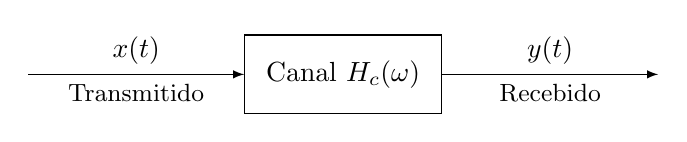
\begin{tikzpicture}[>=latex]
\node[draw, rectangle, minimum width=2.5cm, minimum height=1cm] (canal) at (0,0) {Canal $H_c(\omega)$};
\draw[->] (-4,0) -- node[above] {$x(t)$} node[below] {\small Transmitido} (canal.west);
\draw[->] (canal.east) -- node[above] {$y(t)$} node[below] {\small Recebido} (4,0);
\end{tikzpicture}
\end{center}

\textbf{Relação entrada-saída:}

No tempo: $y(t) = x(t) \conv h_c(t)$

Na frequência: $Y(\omega) = H_c(\omega) X(\omega)$

\vspace{0.3cm}

\textbf{Canal ideal:}
\[
H_c(\omega) = K e^{-j\omega t_d}
\]

Apenas amplifica e atrasa o sinal, sem alterar sua forma.

\vspace{0.3cm}

\textbf{Canal real:} $H_c(\omega)$ tem $|H_c(\omega)|$ e $\phi_c(\omega)$ variáveis, causando distorção.

\end{frame}

% ============================================

\subsection{Tipos de Distorção}

\begin{frame}{Distorção de Amplitude}

\textbf{Causa:} $|H_c(\omega)|$ não é constante na banda do sinal.

\textbf{Efeito:}

Diferentes componentes de frequência são amplificadas/atenuadas diferentemente:

\[
|Y(\omega)| = |H_c(\omega)| \cdot |X(\omega)|
\]

\textbf{Consequências práticas:}

\begin{itemize}
\item Alteração do formato da forma de onda
\item Componentes importantes podem ser atenuadas
\item Interferência entre símbolos (ISI) em comunicação digital
\item Degradação da relação sinal-ruído
\end{itemize}

\textbf{Exemplo típico:}

Canal telefônico: atenuação aumenta com frequência (efeito de cabo)

\[
|H_c(\omega)| \approx e^{-\alpha \omega}
\]

Altas frequências sofrem maior atenuação que baixas frequências.

\end{frame}

% ============================================

\begin{frame}{Exemplo: Distorção de Amplitude}

\textbf{Situação:} Pulso quadrado transmitido através de canal passa-baixas.

Pulso quadrado contém harmônicas ímpares: $\omega_0, 3\omega_0, 5\omega_0, ...$

\textbf{Canal com resposta:}
\[
|H_c(\omega)| = \begin{cases}
1 & |\omega| \leq 3\omega_0 \\
0.5 & 3\omega_0 < |\omega| \leq 5\omega_0 \\
0.1 & |\omega| > 5\omega_0
\end{cases}
\]

\textbf{Efeito na recepção:}

\begin{itemize}
\item Fundamental ($\omega_0$): passa sem alteração
\item 3ª harmônica ($3\omega_0$): atenuada a 50\%
\item 5ª harmônica e superiores: fortemente atenuadas
\end{itemize}

\textbf{Resultado:} Bordas do pulso ficam arredondadas, perdendo "nitidez".

\end{frame}

% ============================================

\begin{frame}{Distorção de Fase}

\textbf{Causa:} $\phi_c(\omega) = \arg[H_c(\omega)]$ não é linear com $\omega$.

\textbf{Condição ideal:}
\[
\phi_c(\omega) = -\omega t_d \quad \text{(fase linear)}
\]

Todas as frequências sofrem o mesmo atraso temporal $t_d$.

\vspace{0.3cm}

\textbf{Fase não-linear:}

Se $\phi_c(\omega) \neq -\omega t_d$, diferentes frequências chegam em tempos diferentes.

\textbf{Consequências:}

\begin{itemize}
\item Distorção da forma de onda mesmo sem distorção de amplitude
\item Componentes do sinal ficam "fora de sincronismo"
\item Especialmente problemático para sinais com muitas componentes espectrais
\item Crítico em comunicação digital (pulsos se dispersam)
\end{itemize}

\end{frame}

% ============================================

\begin{frame}{Atraso de Grupo}

O \textbf{atraso de grupo} mede o atraso de envelopes de sinais:

\[
\tau_g(\omega) = -\frac{d\phi_c(\omega)}{d\omega}
\]

\textbf{Interpretação física:}

\begin{itemize}
\item Para fase linear $\phi = -\omega t_d$: $\tau_g = t_d$ (constante)
\item Todas as componentes de frequência "viajam juntas"
\item Para $\tau_g(\omega)$ variável: dispersão temporal das componentes
\end{itemize}

\vspace{0.3cm}

\textbf{Efeito em sinais modulados:}

Sinal modulado: $x(t) = m(t)\cos(\omega_c t)$

Se $\tau_g$ varia na banda de $m(t)$, o envelope $m(t)$ é distorcido.

\vspace{0.3cm}

\textbf{Especificação de canal:}

Canal aceitável: $\tau_g(\omega)$ aproximadamente constante na banda de interesse.

\end{frame}

% ============================================

\begin{frame}{Exemplo: Distorção de Fase}

\textbf{Sinal:} Soma de duas senoides:

\[
x(t) = \cos(\omega_1 t) + \cos(\omega_2 t)
\]

\textbf{Canal ideal:} $H_c(\omega) = e^{-j\omega t_d}$

\[
y(t) = \cos[\omega_1(t - t_d)] + \cos[\omega_2(t - t_d)]
\]

Ambas componentes atrasadas igualmente $\rightarrow$ forma preservada.

\vspace{0.3cm}

\textbf{Canal com fase não-linear:}

$\phi_c(\omega_1) = -\omega_1 t_1$, $\phi_c(\omega_2) = -\omega_2 t_2$ com $t_1 \neq t_2$

\[
y(t) = \cos[\omega_1(t - t_1)] + \cos[\omega_2(t - t_2)]
\]

Componentes atrasadas diferentemente $\rightarrow$ interferência construtiva/destrutiva em tempos diferentes $\rightarrow$ forma alterada.

\end{frame}

% ============================================

\subsection{Distorção Linear versus Não-Linear}

\begin{frame}{Classificação da Distorção}

\begin{enumerate}
\item \textbf{Distorção Linear:}
   \begin{itemize}
   \item Causada por $|H_c(\omega)|$ variável ou $\phi_c(\omega)$ não-linear
   \item Canal ainda é sistema LTI
   \item Não cria novas frequências
   \item Apenas modifica componentes existentes
   \item \textbf{Pode ser compensada} por equalização linear
   \end{itemize}

\item \textbf{Distorção Não-Linear:}
   \begin{itemize}
   \item Canal não obedece princípio da superposição
   \item Exemplos: saturação, compressão, intermodulação
   \item \textbf{Cria novas frequências} (harmônicas, produtos de intermodulação)
   \item Muito mais difícil de compensar
   \item Requer equalização não-linear ou evitar operação não-linear
   \end{itemize}
\end{enumerate}

\vspace{0.3cm}

\textbf{Foco desta seção:} Distorção linear (mais comum e tratável).

\end{frame}

% ============================================

\subsection{Equalização}

\begin{frame}{Conceito de Equalização}

\textbf{Objetivo:} Compensar a distorção introduzida pelo canal.

\textbf{Princípio:}

Inserir um \textbf{filtro equalizador} $H_{eq}(\omega)$ no receptor que "inverte" o efeito do canal.

\begin{center}
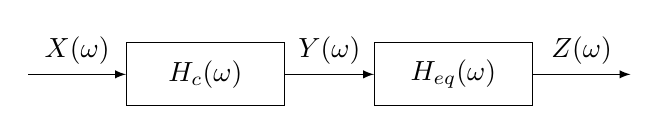
\begin{tikzpicture}[>=latex, scale=0.9]
\node[draw, rectangle, minimum width=2cm, minimum height=0.8cm] (canal) at (0,0) {$H_c(\omega)$};
\node[draw, rectangle, minimum width=2cm, minimum height=0.8cm] (eq) at (3.5,0) {$H_{eq}(\omega)$};
\draw[->] (-2.5,0) -- node[above] {$X(\omega)$} (canal.west);
\draw[->] (canal.east) -- node[above] {$Y(\omega)$} (eq.west);
\draw[->] (eq.east) -- node[above] {$Z(\omega)$} (6,0);
\end{tikzpicture}
\end{center}

\textbf{Função de transferência total:}

\[
Z(\omega) = H_{eq}(\omega) \cdot H_c(\omega) \cdot X(\omega)
\]

\textbf{Condição ideal:}

\[
H_{eq}(\omega) \cdot H_c(\omega) = K e^{-j\omega t_d}
\]

Portanto:
\[
H_{eq}(\omega) = \frac{K e^{-j\omega t_d}}{H_c(\omega)}
\]

\end{frame}

% ============================================

\begin{frame}{Equalização Ideal}

\textbf{Equalizador ideal:}

\[
H_{eq}(\omega) = \frac{1}{H_c(\omega)} = \frac{1}{|H_c(\omega)|} e^{-j\phi_c(\omega)}
\]

\textbf{Efeitos:}

\begin{itemize}
\item \textbf{Equalização de magnitude:} $|H_{eq}(\omega)| = 1/|H_c(\omega)|$
  \begin{itemize}
  \item Frequências atenuadas pelo canal são amplificadas
  \item Frequências amplificadas pelo canal são atenuadas
  \end{itemize}

\item \textbf{Equalização de fase:} $\phi_{eq}(\omega) = -\phi_c(\omega)$
  \begin{itemize}
  \item Cancela a fase não-linear do canal
  \item Restaura relações de fase corretas
  \end{itemize}
\end{itemize}

\vspace{0.3cm}

\textbf{Limitações práticas:}

\begin{itemize}
\item $H_c(\omega)$ deve ser conhecido (estimação de canal)
\item Não pode ser zero em nenhuma frequência (divisão por zero)
\item Amplifica ruído onde $|H_c(\omega)|$ é pequeno
\item Pode ser não-causal se $H_c(\omega)$ não for de fase mínima
\end{itemize}

\end{frame}

% ============================================

\begin{frame}{Tipos de Equalizadores}

\begin{enumerate}
\item \textbf{Equalizador Fixo:}
   \begin{itemize}
   \item Projetado para canal conhecido e estático
   \item Coeficientes fixos
   \item Simples, baixo custo
   \item Exemplo: cabo de comprimento conhecido
   \end{itemize}

\item \textbf{Equalizador Adaptativo:}
   \begin{itemize}
   \item Ajusta coeficientes automaticamente
   \item Rastreia variações do canal
   \item Usa sequência de treinamento ou decisões
   \item Algoritmos: LMS, RLS, CMA
   \item Aplicação: canais móveis, fibra óptica
   \end{itemize}

\item \textbf{Equalizador de Decisão Realimentada (DFE):}
   \begin{itemize}
   \item Usa decisões passadas para cancelar ISI
   \item Não amplifica ruído em frequências com $|H_c| \approx 0$
   \item Mais eficiente em canais com zeros espectrais
   \end{itemize}
\end{enumerate}

\end{frame}

% ============================================

\subsection{Exemplos Práticos}

\begin{frame}{Exemplo 1: Canal Telefônico}

\textbf{Características típicas do canal telefônico (PSTN):}

\begin{itemize}
\item Banda nominal: 300 Hz a 3400 Hz
\item Atenuação: aumenta com frequência (skin effect)
\item Fase: não-linear próximo aos extremos da banda
\item Atraso de grupo: variação de até 2 ms na banda
\end{itemize}

\vspace{0.3cm}

\textbf{Modelo simplificado:}

\[
|H_c(f)| \approx e^{-\alpha f} \quad \text{para} \quad 300 \text{ Hz} < f < 3400 \text{ Hz}
\]

com $\alpha$ dependendo do comprimento do cabo.

\vspace{0.3cm}

\textbf{Equalização:}

Modems de linha discada (V.32, V.34, V.90) usam equalizadores adaptativos complexos para atingir taxas de 28.8-56 kbps nesta banda limitada e distorcida.

\end{frame}

% ============================================

\begin{frame}{Exemplo 2: Canal em Cabo Coaxial}

\textbf{Características de cabo coaxial (TV a cabo, Ethernet):}

\begin{itemize}
\item Atenuação: $\alpha(f) = k_1\sqrt{f} + k_2 f$ (dB/km)
  \begin{itemize}
  \item Termo $\sqrt{f}$: perdas dielétricas
  \item Termo $f$: efeito pelicular (skin effect)
  \end{itemize}
\item Fase: aproximadamente linear
\item Dispersão: mínima em frequências mais baixas
\end{itemize}

\vspace{0.3cm}

\textbf{Exemplo numérico:} RG-59 a 100 MHz e 1 km

Atenuação $\approx 20$ dB $\rightarrow$ $|H_c| \approx 0.1$

\textbf{Equalização:}

Amplificadores em linha com resposta pré-distorcida:

\[
|H_{amp}(f)| \propto \sqrt{f} \quad \text{ou} \quad |H_{amp}(f)| \propto f
\]

Compensa a atenuação crescente do cabo.

\end{frame}

% ============================================

\begin{frame}{Exemplo 3: Canal sem Fio com Multipercurso}

\textbf{Efeito multipercurso:}

Sinal chega ao receptor por múltiplos caminhos com diferentes atrasos e atenuações.

\textbf{Modelo de canal:}

\[
h_c(t) = \sum_{i=1}^{N} a_i \delta(t - \tau_i)
\]

\textbf{Resposta em frequência:}

\[
H_c(\omega) = \sum_{i=1}^{N} a_i e^{-j\omega\tau_i}
\]

\textbf{Características:}

\begin{itemize}
\item \textbf{Desvanecimento seletivo em frequência:} $|H_c(\omega)|$ varia rapidamente
\item Frequências onde há interferência destrutiva: $|H_c(\omega)| \approx 0$ (nulls)
\item Atraso de grupo altamente variável
\item Canal varia com tempo (movimento)
\end{itemize}

\textbf{Equalização:} Adaptativa complexa, OFDM para contornar desvanecimento.

\end{frame}

% ============================================

\begin{frame}{Compromisso: Equalização versus Ruído}

\textbf{Problema fundamental:}

Equalização amplifica sinal \textbf{E} ruído nas frequências atenuadas pelo canal.

\textbf{Análise:}

Canal: $Y(\omega) = H_c(\omega)X(\omega) + N(\omega)$

Após equalização: $Z(\omega) = H_{eq}(\omega)Y(\omega)$

\[
Z(\omega) = H_{eq}(\omega)H_c(\omega)X(\omega) + H_{eq}(\omega)N(\omega)
\]

Se $|H_c(\omega_0)| \approx 0$ (null espectral):

\begin{itemize}
\item Equalizador requer $|H_{eq}(\omega_0)| \to \infty$
\item Ruído nessa frequência é amplificado enormemente
\item SNR deteriora drasticamente
\end{itemize}

\vspace{0.3cm}

\textbf{Solução:} Equalização de mínimo erro quadrático médio (MMSE) que balanceia distorção residual vs. amplificação de ruído.

\end{frame}

% ============================================

\begin{frame}{Resumo da Seção 3.6}

\textbf{Tipos de distorção em canais:}

\begin{itemize}
\item \textbf{Distorção de amplitude:} $|H_c(\omega)|$ variável
\item \textbf{Distorção de fase:} $\phi_c(\omega)$ não-linear
\item Ambas alteram formato do sinal
\end{itemize}

\vspace{0.3cm}

\textbf{Atraso de grupo:} $\tau_g(\omega) = -d\phi_c/d\omega$

Deve ser constante para evitar distorção de fase.

\vspace{0.3cm}

\textbf{Equalização:}

\begin{itemize}
\item Compensa distorção: $H_{eq}(\omega) \approx 1/H_c(\omega)$
\item Pode ser fixa ou adaptativa
\item Compromisso: correção vs. amplificação de ruído
\end{itemize}

\vspace{0.3cm}

\textbf{Aplicações práticas:} Telefonia, TV a cabo, comunicação sem fio.

\end{frame}
